\documentclass[../main.tex]{subfiles}
\begin{document}

\chapter{Lecture 23 - 08-06-2020}
\bred{Bagging}
$$
h_1,...,h_t \qquad \hat{\ell}(f) \leq e^{-2 \, T \gamma^2} \qquad \gamma_t > \gamma>0
$$
Under the assumption that $ \{ h_t(x_z) \neq y_z \} $ \qquad $ \gamma_t = \frac{1}{2} - \hat{\ell}_s(h_t)$ are independent 
$$
f = sgn ( \sum_{i=1}^T h_i) \qquad Bagging
$$
\section{Boosting}
$$
f = sgn ( \sum_{i=1}^T w_i h_i) \qquad Boosting
$$
The hard thing here is how to compute the weights.
\\
$
h_1, ..., h_t \qquad X \rightarrow \{ -1,+1 \} 
$
\begin{figure}[h]
    \centering
    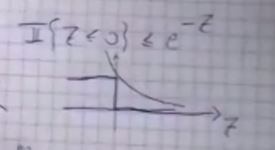
\includegraphics[width=0.3\linewidth]{../img/lez23-img1.JPG}
    \caption{}
    %\label{fig:}
\end{figure}\\
\\
$$
\hat{\ell}(f)\sum^m_{t=1} I \{ y_t g(x_t) \leq 0 \}
\leq
\frac{1}{m} \sum_{t=1}^m e^{-g(x_t) y_t
} = $$
$$
g = \sum_{i = 1}^T w_i h_i \textit{and we substitute g} \qquad and \qquad f = sgn(g)
$$
$$
= \ \frac{1}{m} \sum^m_{t=1} e^{-y_t \, \sum_{t=1}^T w_i h_i(x_i)} \qquad L_i(t) = h_i (x_t) y_t \in \{-1,+1 \} i = 1, ..., T
$$
$
L_i(z) 
$ where $Z$ uniform over $\{1,...,m\}$
$$
\hat(\ell)(f) \leq \frac{1}{m} \sum_{t=1}^m e^{- \sum_{t=1}^T w_i L_i (t)} = \barra{E} \left[ e^{-\sum_{t=1}^T w_i L_i (t)}\right] 
$$
$$
\barra{E} \left[ \prod_{t=1}^T e^{- w_i L_i}\right] =^? \prod^T_{t=1} \barra{E} \left[ e^{-w_i Li} \right]
$$
Ok if $Li$ are independent
\\$E\left[XY \right] = \barra{E}[X] \, \barra{E} [Y]$ 
\\
$X,Y$ are independent
\\
$\barra{E}_i $ is a probability $P_i$ and $P_i$ is sum $\{1,...m\}$
\\
$$
\hat{\ell}(f)\ \leq \ \prod_{i=1}^T \barra{E}_i \left[ e^{- w_i L_i} \right]
\ = \ \prod_{i=1}^T \left( e^{w_i} P_i (L_i = 1) + e^{w_i} P_i\left(L_i=1  \right) \right) \ = \ \prod_{i=1}^T \left( e^{-w_i}(1 - \epsilon_i) + e^{-w_i} \varepsilon_i \right)$$
$ L_i(z) \qquad z \sim P_i$
$$
\varepsilon_i = P_i(L_i = -1) = \sum_{t=1}^m I \{y_t h_i(x_t) \leq 0 \} P_i(t) \qquad \textbf{weighted training error of $h_i$}
$$
$$
F(w) = e^{-w} (1- \varepsilon) + e^w \varepsilon \qquad F'(w) = 0 \Leftrightarrow w = \frac{1}{2} \ln \frac{1-\varepsilon}{\varepsilon} \qquad 0< \varepsilon< 1
$$
$$
P_i(t) > 0 \quad \forall i,t \qquad \varepsilon_i = \frac{1}{2} \Rightarrow w_i = 0
$$
$$
\varepsilon_i >\frac{1}{2} \Rightarrow w_i < 0 \qquad \qquad
\varepsilon_i < \frac{1}{2} \Rightarrow w_i > 0
$$

$$
\hat{\ell}(f) \ \leq \ \prod_{i=1}^T \sqrt[]{4 \, \varepsilon_i (1-\varepsilon_i)}
$$
$$
\gamma_i = \frac{1}{2} - \varepsilon_i \qquad  \textit{edge over random guessing $ 0 < \varepsilon_i <1$}
$$
$$
1 + x \leq e^x \quad \forall x \in \barra{R} \quad \hat{\ell}(f) \leq \prod_{i=1}^T \sqrt[]{4 \, \varepsilon_i(1 - \varepsilon_i)} \ = \
\prod_{i=1}^T \sqrt[]{1- 4 \gamma^2} = 
$$
$$\ = \ \prod_{i = 1}^T 4 (\frac{1}{2} - \gamma_i)(\frac{1}{2}+ \gamma_i) \ = \prod_{i=1}^T e^{- 2 \gamma_i^2}  = e^{- 2 \sum_{i=1}^T \gamma_i^2} \leq e^{-2 T \gamma^2}
$$
$
If \quad |\gamma_i| > \gamma > 0 \quad i = 1, ..., T$
$$
\hat{\ell}_s(f) = 0 \ \Leftrightarrow \ e^{-\varepsilon T \gamma^2}< \frac{1}{m} \ \Leftrightarrow \ T > \frac{ \ln m}{2 \gamma^2}
$$
$$
E \left[ \prod_i e^{-w_i L_i }\right] \ = \ \prod_i E \left[ e^{-w_i L_i } \right]
$$
$P_i,...,P_T \quad P_1(t) = \frac{1}{m}$ \quad $ t = 1,...m$
$$
P_{i+1}(t) = \frac{P_i(t) e^{-w_i L_i(t)}}{E_i \left[ e^{-w_i L_i} \right] } \qquad \sum_t P_{i+1}(t) = \frac{1}{E_i [e^{-w_i L_i}]} 
\sum_t P_i(t) e^{...}
$$
MANCAaaa
$$
e^{-w_i L_i(t)} = E_i [e^{-w_i L_i}] \frac{P_{i+1}}{P_i(t)}
$$
$$
E[\prod_{i=1}^T e^{-w_i L_i}] = \frac{1}{m} \sum_{t=1}^m \prod_{i=1}^T e^{-w_i L_i(t)} = \frac{1}{m} \sum_t l\left( \prod_i E [e^{- w_i L_i}] \frac{P_{t+1}(t)}{P_i(t)}\right) \ = 
$$
$$
\frac{1}{m} \sum_t \left( \prod_i E_i [e^{-w_i L_i} \right) \frac{P_{t+1}(t)}{P_1(t)} = \left( \prod_i E_i[e^{-w_i L_i}] \right) \red{\frac{1}{m} \sum_t \frac{P_{t+1}(t)}{y m}}
$$
where \bred{red} cancel out since $= 1$
\newpage
\section{Adaboost}
It is a meta learning algorithm.
\begin{figure}[h]
    \centering
    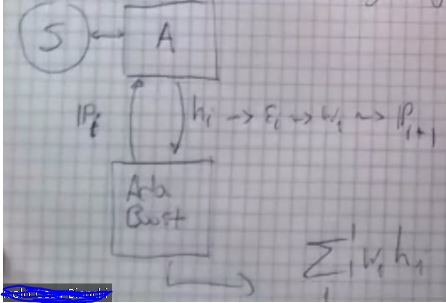
\includegraphics[width=0.5\linewidth]{../img/lez23-img2.JPG}
    \caption{}
    %\label{fig:}
\end{figure}\\
\\
Initialize $P_i(t) = \frac{1}{m} \quad t=1,...,m$\\
For $i = 1,...,T$\\
1) Feed $A$ with $S$ wrighted by $P_i$ and get $h_1$\\
2) $w_i = \frac{1}{2} \ln \frac{\varepsilon_i}{1-\varepsilon_i}$
\\
3) Compute $P_{i+1}$
\\
Output $\sum_i w_i h_i$
\\\\
What should $A$ do? \\
1) $A$ should pay attention to $P_i$ \\
2) More precisely $A$ should output $h_i$ s.t. $|\gamma_i|$ is as big as possible  \\ where $ | \gamma | \rightarrow \frac{1}{2} \varepsilon_i$ 
\begin{figure}[h]
    \centering
    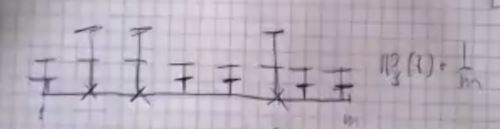
\includegraphics[width=0.5\linewidth]{../img/lez23-img3.JPG}
    \caption{}
    %\label{fig:}
\end{figure}\\
$$
P_{i+1}= \frac{P_i(t) e^{-w_i L_i(t)} }{E_i[ \quad ]}
$$
$$
L_i(t) = 1 \ \Leftrightarrow h_t(x_t) = y_t \qquad w_i > 0
$$ 
\\
\begin{figure}[h]
    \centering
    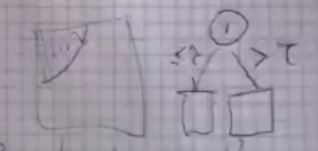
\includegraphics[width=0.3\linewidth]{../img/lez23-img4.JPG}
    \caption{}
    %\label{fig:}
\end{figure}\\
Typically $h_i$ (classifiers) are simple
\\
\bred{Decision stamps}:
$$
h(x) = \pm \ sgn (x_i- \tau)
$$
$i$ if is feature index, $\tau \in \barra{R}$\\
At the end boosting is gonna look like this
\\
\begin{figure}[h]
    \centering
    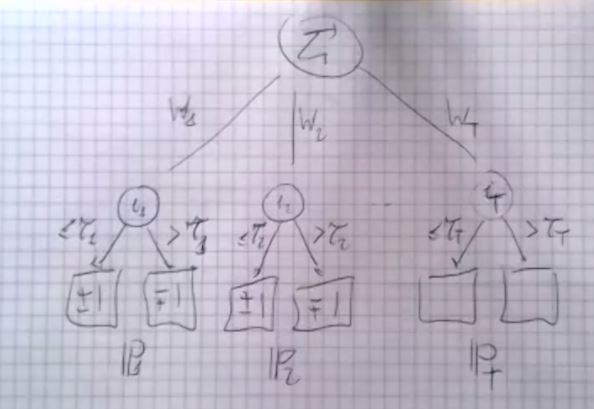
\includegraphics[width=0.5\linewidth]{../img/lez23-img5.JPG}
    \caption{}
    %\label{fig:}
\end{figure}\\
\end{document}